\documentclass{beamer}
\usepackage[utf8]{inputenc}
\usepackage{verbatim}
\usepackage{hyperref}

\usetheme{Copenhagen}
\usecolortheme{beetle}


\title{Introdução ao \LaTeX}
\subtitle{Uso básico e Classe \LaTeX~FEI}
\author{Rodrigo Prior Bechelli}
\institute{Centro Universitário da FEI}
\date[SP 2016] % (optional)
{Electrical Engineering, Signal Processing, 2016}
\logo{
\includegraphics[height=.8cm]{logo_fei}}

\begin{document}

\begin{frame}
    \titlepage
\end{frame}

\AtBeginSection[]
{
  \begin{frame}
    \frametitle{Outline}
    \tableofcontents[currentsection]
  \end{frame}
}

\section{Intro}


\begin{frame}{O que é?}
    \begin{itemize}
        \item \TeX~(``tech'') é uma linguagem de programação (\emph{typesetting language}) criada em 1978 por Donald E. Knuth (``The Art of Computer Programming'')\dots
        \item \LaTeX~(``Lay-tech'' ou ``Lah-tech'') é um conjunto de macros para formatação de arquivos baseada em \TeX~desenvolvido em 1985 por Leslie Lamport (\url{https://latex-project.org}).
        \item É uma linguagem de programação para criar documentos.
        \item Simplifica a geração de equações, índice de páginas, índice de figuras, índice de tabelas, inserção de referências bibliográficas entre outros\dots
        \item Promove uma isolação entre conteúdo e estílo.
    \end{itemize}
\end{frame}


\begin{frame}{O que NÃO é?}
    \begin{itemize}
        \item Não é um editor de texto.
        \item Não é um editor visual.
        \item Não é um gerador de graficos ou tabelas.
        \item Não é uma solução rápida ou um quebra galho.
    \end{itemize}
\end{frame}


\begin{frame}{Quem usa?}
    \begin{itemize}
        \item IEEE - \url{http://www.ieee.org/documents/IEEEtran.zip}
        \item NASA - \url{http://www.giss.nasa.gov/tools/latex/}
        \item Elsevier - \url{https://www.elsevier.com/authors/author-schemas/latex-instructions}
        \item Wiley - \url{http://exchanges.wiley.com/authors/wiley-latex-template_766.html}
        \item Springer - \url{https://www.springer.com/gp/authors-editors/book-authors-editors/manuscript-preparation/5636}
        \item Submissão de Congressos\dots
    \end{itemize}
\end{frame}

\section{Como Programar}

\subsection{Conceitos Básicos}

\begin{frame}{O que é necessário para programar \LaTeX?}
    \begin{itemize}
        \item Editor de texto
        \begin{itemize}
            \item Sublime Text 3
            \item Atom
            \item TexMaker
        \end{itemize}
        \item Compilador \LaTeX~
        \begin{itemize}
            \item pdflatex: .tex para .pdf
        \end{itemize}
    \end{itemize}
\end{frame}


\begin{frame}{Divisões}
    \begin{columns}[T]
        \begin{column}{.5\textwidth}
            \begin{block}{}
                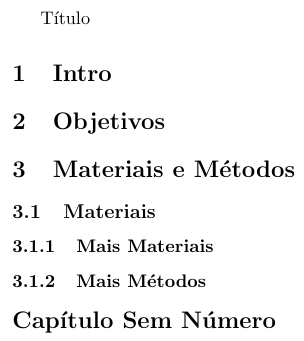
\includegraphics[width=\columnwidth]{divisoes_output}
            \end{block}
        \end{column}
        \begin{column}{.5\textwidth}
            \begin{block}{}
                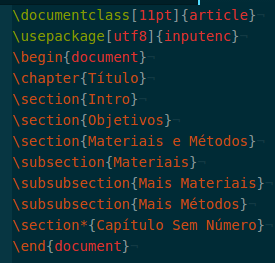
\includegraphics[width=\columnwidth]{divisoes_codigo}
            \end{block}
        \end{column}
    \end{columns}
\end{frame}


\begin{frame}{Equações}
    Código:
    \begin{figure}[!htb]
        \begin{center}
            \label{fig:equation_ex}
            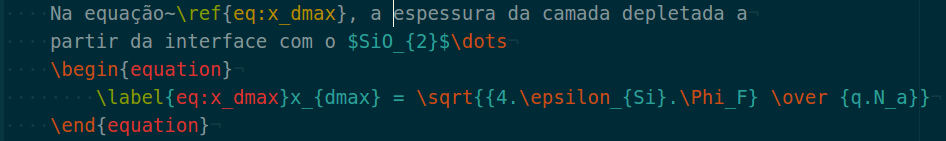
\includegraphics[width=\columnwidth]{equation}
        \end{center}
    \end{figure}
    %
    \rule{\textwidth}{1pt}
    Na equação~\ref{eq:x_dmax}, a espessura da camada depletada a
    partir da interface com o $SiO_{2}$\dots
    \begin{equation}
        \label{eq:x_dmax}x_{dmax} = \sqrt{{4.\epsilon_{Si}.\Phi_F} \over {q.N_a}}
    \end{equation}
\end{frame}


\begin{frame}{Tabelas}
    \begin{columns}[T]
        \begin{column}{.5\textwidth}
            \begin{block}{}
                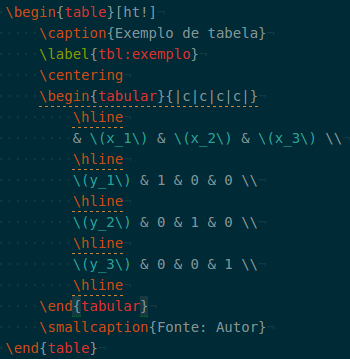
\includegraphics[width=\columnwidth]{tabela}
            \end{block}
        \end{column}
        \begin{column}{.5\textwidth}
            \begin{block}{}
                \begin{table}[ht!]
                    \caption{Exemplo de tabela}
                    \label{tbl:exemplo}
                    \centering
                    \begin{tabular}{|c|c|c|c|}
                        \hline
                        & \(x_1\) & \(x_2\) & \(x_3\) \\
                        \hline
                        \(y_1\) & 1 & 0 & 0 \\
                        \hline
                        \(y_2\) & 0 & 1 & 0 \\
                        \hline
                        \(y_3\) & 0 & 0 & 1 \\
                        \hline
                    \end{tabular}\\
                    \smallcaption{Fonte: Autor}
                \end{table}
            \end{block}
        \end{column}
    \end{columns}
\end{frame}


\begin{frame}[fragile]{Figuras}
    \begin{figure}
        \centering
        \caption{Exemplo de figura com sua fonte.}
        
\includegraphics[height=1.5cm]{logo_fei}\\
        \smallcaption{Fonte: Autor.}\label{fig:exemplo}
    \end{figure}
    Código-fonte:
    \begin{verbatim}
        \begin{figure}
            \centering
            \caption{Exemplo de figura com sua fonte.}
            \includegraphics[...]{...}
            \smallcaption{Fonte: Autor.}
        \end{figure}
    \end{verbatim}
\end{frame}


\begin{frame}
    Alguns links de editores online que podem ser utilizados:
    \begin{itemize}
        \item  \url{https://www.overleaf.com/}
        \item  \url{https://www.sharelatex.com/}
        \item  \url{https://papeeria.com/}
    \end{itemize}
\end{frame}


\section{Referências Bibliográficas}

\begin{frame}{Introdução}
    \begin{itemize}
        \item \LaTeX~possui um gerenciamento automático de referências bibliográficas.
        \item Existem diversos pacotes que podem ser utilizados, os mais comuns são:
        \begin{itemize}
            \item natbib (\url{http://ctan.org/pkg/natbib})
            \item abnTeX (\url{http://www.abntex.net.br/})
        \end{itemize}
    \end{itemize}
\end{frame}


\begin{frame}{Como Gerenciar Referências Bibliográficas}
    Ferramentas para gerenciar referências bibliográficas:
    \begin{itemize}
        \item JabREF – Linux/Win/OSX
        \item Mendeley – Online/Linux/Win/OSX
        \item Zotero – Online/Linux/Win/OSX
        \item entre outros\dots
    \end{itemize}
\end{frame}

\begin{frame}
    \begin{center}
        Arquivo .bib:
        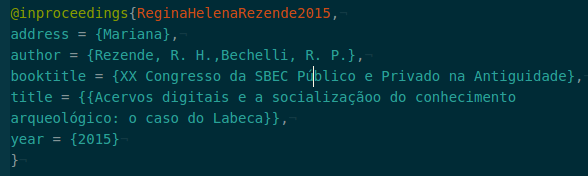
\includegraphics[width=.8\columnwidth]{bibliografia_bib}\\
        Arquivo .tex:
        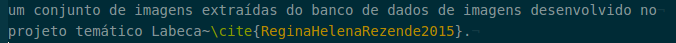
\includegraphics[width=.8\columnwidth]{bibliografia_texto}\\
        Arquivo .pdf:
        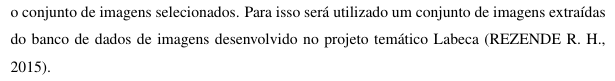
\includegraphics[width=.8\columnwidth]{bibliografia_output}\\
        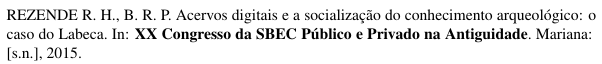
\includegraphics[width=.8\columnwidth]{bibliografia_bibtexto}\\
    \end{center}
\end{frame}


\section{Classe \LaTeX~FEI}

\begin{frame}{Origem da Classe \LaTeX~FEI}
    Extraído do manual da classe:

    ``Guiados por este manual (e mais uma dezena de dissertações corrigidas pelas bibliotecárias), nasceu o arquivo fei.cls, uma classe de documentos \LaTeX~especializada na criação de trabalhos acadêmicos para alunos da FEI. Com ela, os alunos podem utilizar seus conhecimentos em \LaTeX~para criar seus documentos, deixando a formatação complexa do documento a cargo da classe.''
\end{frame}


\begin{frame}{Origem}
    \begin{itemize}
        \item  \url{https://github.com/OpenFEI/Classe-Latex-FEI/}
        \item Menção Honrosa ao MsC. Douglas Rizzo.
        \item First Commit: Feb 8, 2013 (Fonte: GitHub)
        \item Inspirado nas diversas normas ABNT para produção de trabalhos acadêmicos
        \item Baseado no guia da biblioteca do Centro Universitário da FEI
        \item Bastante utilizado na pós-graduação, mas pouco difundido no restante da universidade.
    \end{itemize}
\end{frame}


\begin{frame}{Code Time}
    Mão na massa!!!
\end{frame}


\begin{frame}
    Referências:
    \begin{itemize}
        \item \url{http://ctan.org/}
        \item \url{http://www.latex-project.org/intro.html}
        \item \url{http://www.physics.usyd.edu.au/~hancock/files/presentations/LaTeX-2013-PJH.pptx}
        \item \url{https://www.sharelatex.com/learn/Main_Page}
        \item \url{https://github.com/OpenFEI/Classe-Latex-FEI/}
    \end{itemize}
\end{frame}


\begin{frame}
    \frametitle{Contato}
    \begin{center}
        Rodrigo Prior Bechelli \\
        rodrigo@bechelli.org \\
        \url{http://bechelli.org} \\
        \url{https://github.com/rodrigoprior}
    \end{center}
\end{frame}

\end{document}
